\section{Results}
\label{sec:results}

We report the validity of the proxy (RQ2), the behavior of the searches and the test comparison of the three arms (RQ1), and the change from studio to real-world and Indian photographs (RQ3); interpretation follows in Section~\ref{sec:discussion}.

\subsection{Proxy Validity}
\label{subsec:res-proxy}

The proxy passed the check fixed before the \genone searches (Section~\ref{subsec:proxy}): the Spearman rank correlation between the proxy and the 40-epoch medium scores is $\rho = 0.976$ ($n = 8$), well above the pass threshold of 0.6 (Table~\ref{tab:proxy}, Fig.~\ref{fig:proxy}). The two rankings differ only by a swap of the adjacent lhs3 and lhs5. The same four settings lead both rankings, with the defaults second behind lhs4 on both, but their medium scores lie within 0.026 of each other, so the proxy separates poor settings from good ones far more clearly than good ones from each other.

\begin{table}[!t]
\centering
\caption{Proxy-Validity Check (\genone, Validation \mapfifty)}
\label{tab:proxy}
\footnotesize
\begin{tabular}{@{}lcccc@{}}
\toprule
Setting & Proxy & Rank & Medium & Rank \\
\midrule
lhs1 & 0.08687 & 1 & 0.28423 & 1 \\
lhs2 & 0.23077 & 2 & 0.49451 & 2 \\
lhs3 & 0.29495 & 3 & 0.56712 & 4 \\
lhs5 & 0.30186 & 4 & 0.55195 & 3 \\
lhs7 & 0.37560 & 5 & 0.61246 & 5 \\
lhs6 & 0.44285 & 6 & 0.62161 & 6 \\
Defaults & 0.47648 & 7 & 0.62884 & 7 \\
lhs4 & 0.49547 & 8 & 0.63839 & 8 \\
\midrule
\multicolumn{5}{@{}l@{}}{Spearman $\rho = 0.976$, $n = 8$; pass threshold $\rho \ge 0.6$} \\
\bottomrule
\end{tabular}
\\[2pt]
\parbox{\columnwidth}{\footnotesize Proxy: 12 epochs on the stratified 40\% training subset. Medium: 40 epochs on the full training split. Both at 416~px; rank 1 is the lowest score. lhs1--lhs7 are the Latin hypercube settings.}
\end{table}

\begin{figure}[!t]
\centering
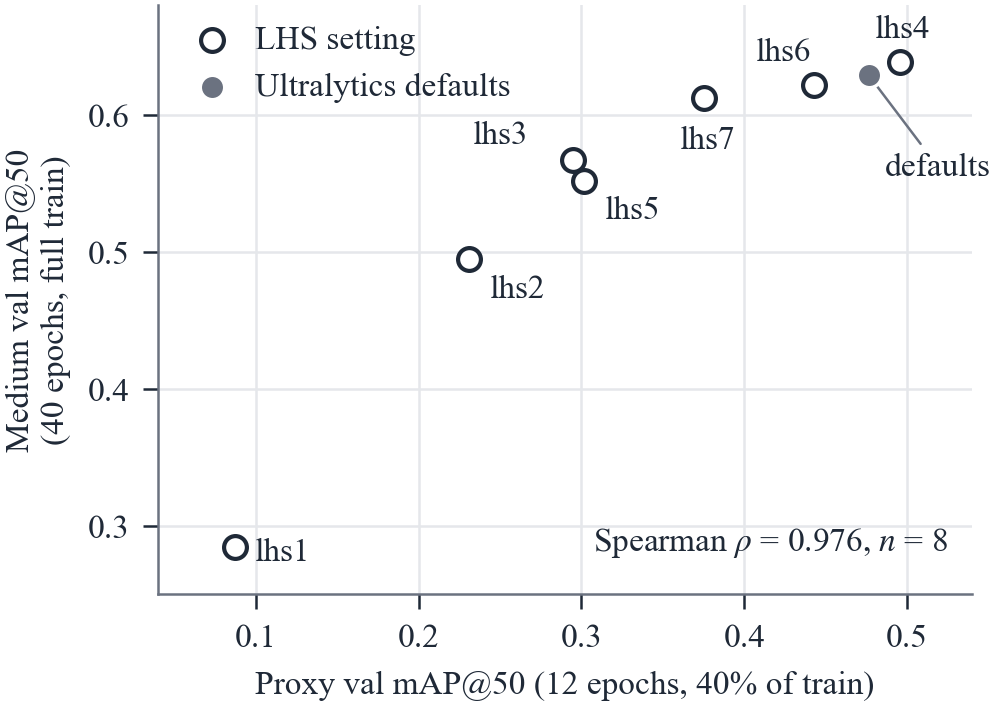
\includegraphics[width=\columnwidth]{r_proxy.png}
\caption{Proxy versus medium validation \mapfifty for the eight settings of the \genone proxy-validity check. The rankings agree except for the adjacent pair lhs3 and lhs5.}
\label{fig:proxy}
\end{figure}

A second, indirect check uses configurations that both generations evaluated. With the same seeds and search space, random search drew the same 32 configurations in both generations. PSO's positions depend on the fitness only through the personal and global bests, which coincided long enough for the swarm to visit identical positions in rounds 1--3 (24 evaluations) but not in round~4. On these repeated configurations, the proxy scores of the two generations have Spearman correlations of 0.991 (random search) and 0.892 (PSO), recomputed from the four search logs. This compares proxy with proxy, not proxy with longer training: the generations order settings alike, but this does not replace a proxy-validity check for \gentwo.

\subsection{Search Behavior}
\label{subsec:res-search}

Fig.~\ref{fig:convergence} shows every proxy evaluation and the best score so far. In \genone, random search found its best setting (0.4995 proxy \mapfifty) at its second evaluation and never improved on it. PSO improved in steps, from 0.4894 after round~1 to 0.4942 after round~3 and 0.4953 in round~4 (evaluation 27), and the swarm converged as intended: the round means rose from 0.393 to 0.423, 0.450 and 0.482, and the within-round standard deviation fell from 0.122 to 0.088, 0.047 and 0.011. The defaults scored 0.4765 on the same proxy, above 28 of the 32 random-search and 21 of the 32 PSO evaluations. The two winners differ by only 0.0042, and lhs4 of the proxy check (0.4955) lies between them. All four search winners of the two generations use a smaller initial learning rate than the default of 0.01 (0.0025 to 0.0070).

\begin{figure*}[!t]
\centering
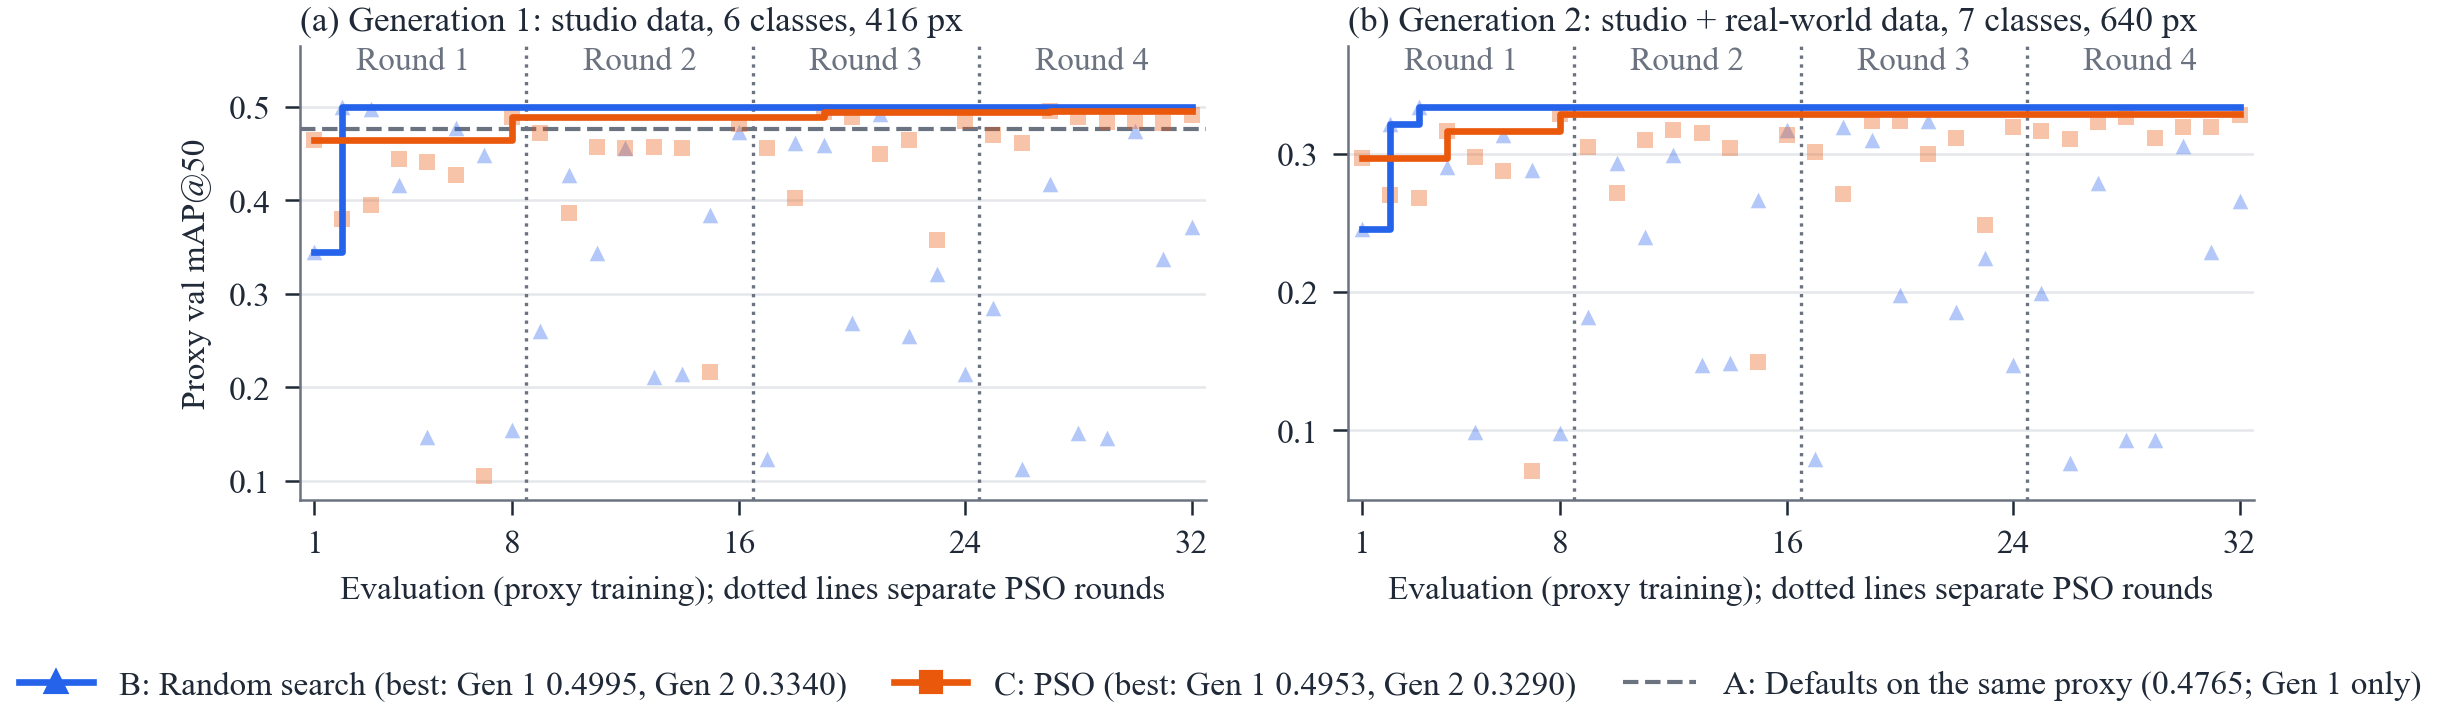
\includegraphics[width=\textwidth]{r_convergence.png}
\caption{Search convergence on the proxy fitness (validation \mapfifty after 12 epochs on 40\% of the training split). Pale markers are individual evaluations (triangles: random search; squares: PSO); solid lines are the best score so far. Dotted lines separate the four PSO rounds of eight particles; random search has no rounds and is plotted in sampling order. The dashed line in (a) is the score of the defaults on the same proxy; \gentwo has no such run. Proxy scores are not comparable between the panels, because the validation sets, classes and image sizes differ.}
\label{fig:convergence}
\end{figure*}

In \gentwo, random search again peaked early (0.3340 at evaluation~3). PSO's best, 0.3290, was the last particle of round~1 and was never beaten (round bests 0.3176, 0.3237 and 0.3279 afterwards), although the swarm still converged: the round means rose from 0.267 to 0.286, 0.300 and 0.319, and the within-round standard deviation fell from 0.082 to 0.006. In both generations, PSO's mean proxy score over all 32 evaluations exceeded that of random search (\genone 0.437 against 0.333; \gentwo 0.293 against 0.226), which reflects the swarm concentrating its later evaluations near good points rather than finding better ones. \gentwo has no proxy run of the defaults, so their standing on the \gentwo proxy is unknown.

\subsection{Generation~1 Test Results (Studio Data)}
\label{subsec:res-gen1}

Table~\ref{tab:gen1-test} gives the one-time test results of the three \genone models on the 1,046 studio test images (7,415 boxes as counted by the evaluator; Table~\ref{tab:datasets} lists 7,413 because it leaves out 2 zero-size boxes). The arms score 0.676 (A), 0.672 (B) and 0.668 (C) \mapfifty, and every pairwise 95\% interval contains 0 on both metrics; the largest difference is C$-$A, $-0.008$ [$-0.021$, $+0.007$]. On studio data, the three arms are therefore statistically tied, and the point estimates even place the defaults first and PSO last; precision and recall are nearly identical. Validation points the same way: the defaults and PSO both reached 0.657, while random search, whose setting had the highest \genone proxy score, reached the lowest value, 0.643.

\begin{table*}[!t]
\centering
\caption{\genone Test Results on the Studio Test Split (1,046 Images)}
\label{tab:gen1-test}
\footnotesize
\begin{tabular}{@{}lcccccc@{}}
\toprule
Arm & Val \mapfifty & Test \mapfifty [95\% CI] & Test \mapfiftyninetyfive [95\% CI] & P & R & ms/img \\
\midrule
A: Defaults & 0.657 & 0.676 [0.639, 0.722] & 0.474 [0.441, 0.518] & 0.747 & 0.581 & 31.4 \\
B: Random search & 0.643 & 0.672 [0.634, 0.717] & 0.475 [0.441, 0.519] & 0.746 & 0.587 & 38.3 \\
C: PSO & 0.657 & 0.668 [0.627, 0.717] & 0.471 [0.437, 0.516] & 0.747 & 0.586 & 31.7 \\
\bottomrule
\end{tabular}
\\[6pt]
\begin{tabular}{@{}lccccc@{}}
\toprule
Pair & $\Delta$\mapfifty [95\% CI] & $P(\Delta>0)$ & $\Delta$\mapfiftyninetyfive [95\% CI] & $P(\Delta>0)$ & Verdict \\
\midrule
B$-$A & $-0.004$ [$-0.016$, $+0.009$] & 0.30 & $+0.001$ [$-0.008$, $+0.010$] & 0.59 & not significant \\
C$-$A & $-0.008$ [$-0.021$, $+0.007$] & 0.16 & $-0.003$ [$-0.012$, $+0.007$] & 0.34 & not significant \\
C$-$B & $-0.004$ [$-0.015$, $+0.007$] & 0.24 & $-0.003$ [$-0.011$, $+0.004$] & 0.19 & not significant \\
\bottomrule
\end{tabular}
\\[2pt]
\parbox{\textwidth}{\footnotesize Val: best checkpoint on the validation split after 100 epochs. CIs: 1,000 paired bootstrap resamples of the test images. P and R at the confidence of maximum F1. ms/img: median batch-1 latency at 416~px on a laptop CPU (Intel Core Ultra~5 125H). $P(\Delta>0)$: share of resamples in which the first arm of the pair scored higher. A difference is significant only if its CI excludes 0.}
\end{table*}

Per class (Fig.~\ref{fig:gen1-perclass}; per-class AP has no confidence interval, Section~\ref{subsec:eval}), the arms differ by less than 0.02 AP@50 on five of the six classes. The exception is PLASTIC, where PSO scores 0.638 against 0.699 (A) and 0.693 (B); PSO is highest on BIODEGRADABLE, GLASS and METAL. The three networks share one architecture, so the higher CPU latency of B (Table~\ref{tab:gen1-test}) most likely reflects other load on the laptop during timing.

\begin{figure}[!t]
\centering
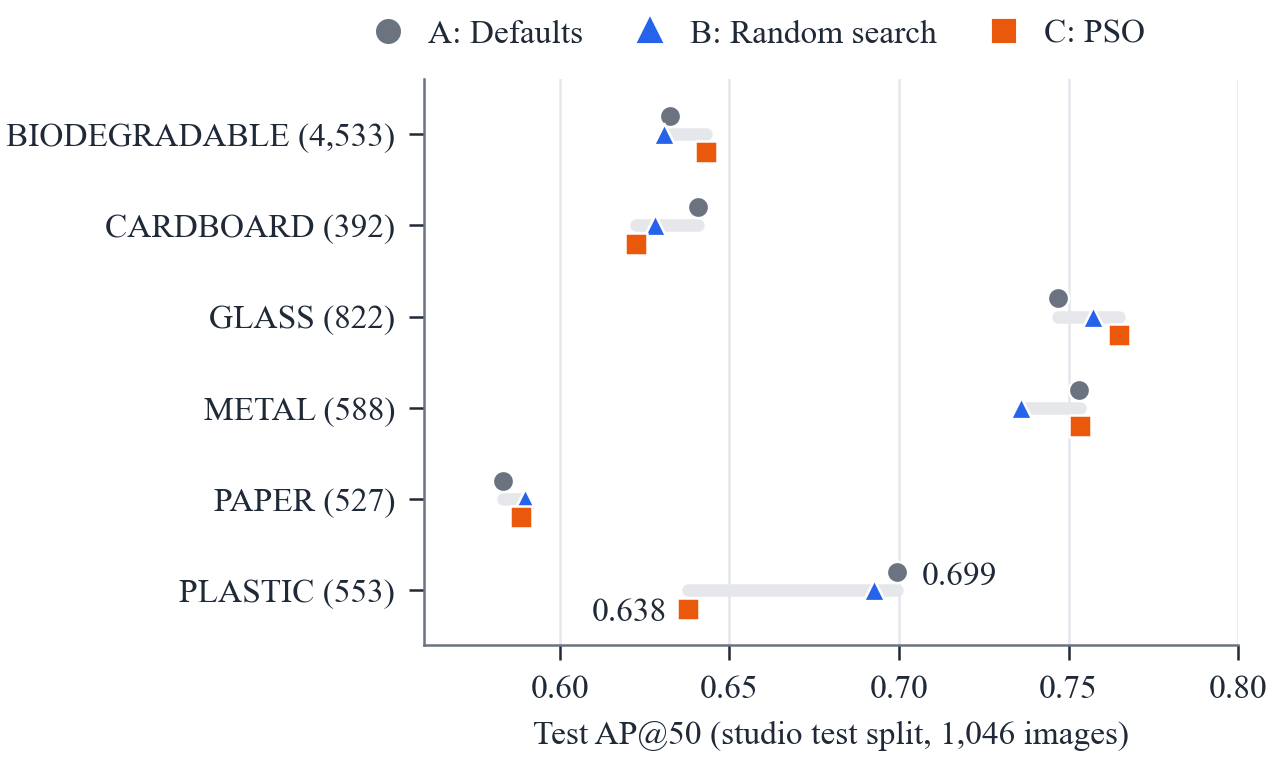
\includegraphics[width=\columnwidth]{r_gen1_per_class.png}
\caption{Per-class test AP@50 of the three \genone models on the studio test split. Numbers in parentheses are the test boxes per class as counted by the evaluator (7,415 in total, including 2 zero-size BIODEGRADABLE boxes); the gray bar spans the three arms' values. PSO is lowest on PLASTIC; elsewhere the arms are within 0.02 of each other.}
\label{fig:gen1-perclass}
\end{figure}

\subsection{Generation~2 Test Results (Mixed Data)}
\label{subsec:res-gen2}

Table~\ref{tab:gen2-test} reports the one-time \gentwo test results on the whole test split and on each domain. On the whole split, the defaults score 0.479, random search 0.497 and PSO 0.500 \mapfifty. Both tuned arms are significantly better than the defaults (B$-$A $+0.017$ [$+0.006$, $+0.030$], C$-$A $+0.020$ [$+0.011$, $+0.032$]), whereas PSO and random search cannot be told apart (C$-$B $+0.003$ [$-0.008$, $+0.015$]). The single-arm intervals overlap widely; the gains are resolved only because the paired bootstrap cancels the variation in image difficulty that all three models share. The \mapfiftyninetyfive verdicts agree with the \mapfifty verdicts everywhere. Random search led PSO on validation (0.473 against 0.466), but on test the two tie.

Studio images contribute 7,413 of the 8,192 boxes, and the studio test set alone (the 1,046 \genone test images) gives the same picture: B$-$A ($+0.024$) and C$-$A ($+0.019$) are significant, C$-$B ($-0.005$) is not. PSO and random search thus differ significantly only on the Indian test set, where all scores are near zero (Section~\ref{subsec:res-domain}).

\begin{table*}[!t]
\centering
\caption{\gentwo Test Results per Test Set: \mapfifty and \mapfiftyninetyfive [95\% CI] per Arm, and Pairwise Differences in \mapfifty}
\label{tab:gen2-test}
\footnotesize
\begin{tabular}{@{}lcccc@{}}
\toprule
 & All & Studio & Real-world & India (DWSD) \\
 & 1,514 img., 8,192 boxes & 1,046 img., 7,413 boxes & 468 img., 779 boxes & 700 img., 4,502 boxes \\
\midrule
\multicolumn{5}{@{}l}{\textit{Test \mapfifty [95\% CI]}} \\
A: Defaults & 0.479 [0.453, 0.513] & 0.571 [0.529, 0.619] & 0.310 [0.278, 0.440] & 0.027 [0.024, 0.031] \\
B: Random search & 0.497 [0.471, 0.531] & 0.595 [0.557, 0.639] & 0.298 [0.271, 0.407] & 0.023 [0.021, 0.027] \\
C: PSO & 0.500 [0.474, 0.534] & 0.590 [0.550, 0.635] & 0.310 [0.279, 0.415] & 0.027 [0.024, 0.031] \\
\midrule
\multicolumn{5}{@{}l}{\textit{$\Delta$\mapfifty [95\% CI] (bold: significant, CI excludes 0)}} \\
B$-$A & $\mathbf{+0.017}$ [$+0.006$, $+0.030$] & $\mathbf{+0.024}$ [$+0.009$, $+0.038$] & $-0.012$ [$-0.118$, $+0.053$] & $\mathbf{-0.003}$ [$-0.006$, $-0.001$] \\
C$-$A & $\mathbf{+0.020}$ [$+0.011$, $+0.032$] & $\mathbf{+0.019}$ [$+0.005$, $+0.033$] & $+0.001$ [$-0.111$, $+0.065$] & $+0.000$ [$-0.003$, $+0.003$] \\
C$-$B & $+0.003$ [$-0.008$, $+0.015$] & $-0.005$ [$-0.018$, $+0.009$] & $+0.013$ [$-0.015$, $+0.036$] & $\mathbf{+0.003}$ [$+0.001$, $+0.006$] \\
\midrule
\multicolumn{5}{@{}l}{\textit{Test \mapfiftyninetyfive [95\% CI]}} \\
A: Defaults & 0.329 [0.309, 0.358] & 0.386 [0.356, 0.425] & 0.254 [0.224, 0.371] & 0.015 [0.013, 0.018] \\
B: Random search & 0.342 [0.322, 0.372] & 0.404 [0.374, 0.442] & 0.238 [0.213, 0.330] & 0.013 [0.012, 0.015] \\
C: PSO & 0.343 [0.323, 0.374] & 0.398 [0.367, 0.439] & 0.248 [0.220, 0.336] & 0.015 [0.013, 0.017] \\
\bottomrule
\end{tabular}
\\[2pt]
\parbox{\textwidth}{\footnotesize All test sets were scored once, at 640~px, with 1,000 paired bootstrap resamples per test set. ``All'' is the whole \gentwo test split (studio plus real-world); India is DWSD, used for testing only. The \mapfiftyninetyfive differences give the same verdict as the \mapfifty differences in every cell. Validation \mapfifty: A 0.454, B 0.473, C 0.466.}
\end{table*}

Per class on the whole split, PSO has the highest AP@50 on five of the seven classes, random search on BIODEGRADABLE and PLASTIC, and the defaults on none. OTHER is very weak for every arm (AP@50 0.050--0.063); all 132 OTHER test boxes are in the real-world images. Precision rises from 0.549 (A) to 0.563 (B) and 0.582 (C), and recall from 0.445 (A) to 0.470 for both tuned arms. The median latency on the T4 at 640~px is 8.1 to 8.7~ms per image.

\subsection{Domain Gap}
\label{subsec:res-domain}

Averaged over the three \gentwo arms, test \mapfifty falls from about 0.59 on studio images to 0.31 on real-world and 0.03 on Indian images (Fig.~\ref{fig:domains}); for every arm, the real-world score is roughly half the studio score.

\begin{figure}[!t]
\centering
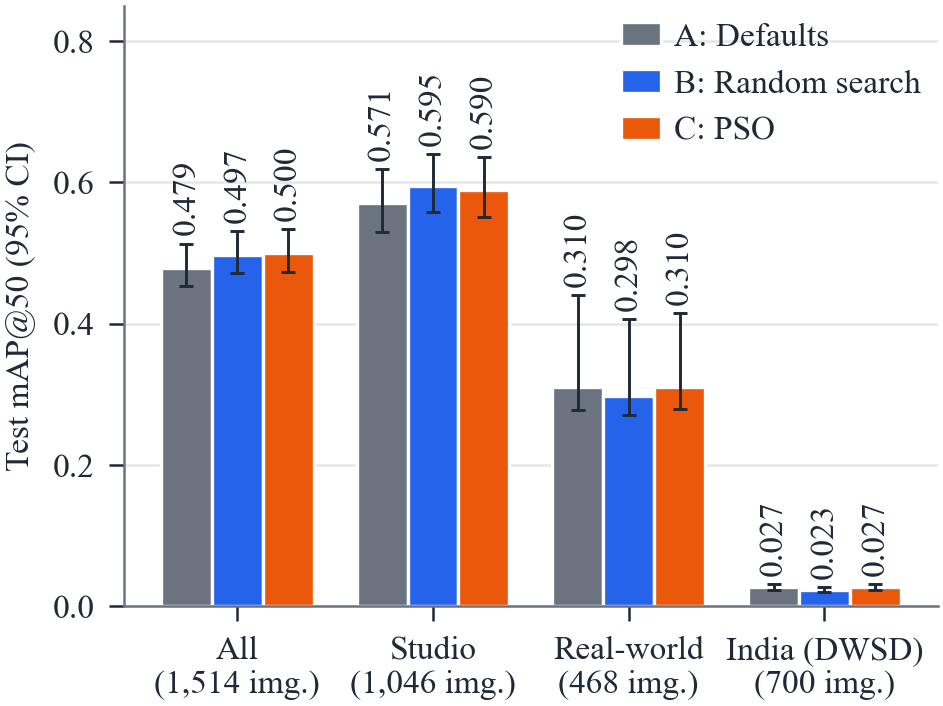
\includegraphics[width=\columnwidth]{r_domains.png}
\caption{Test \mapfifty of the three \gentwo models per test set, with 95\% paired-bootstrap confidence intervals. ``All'' combines the studio and real-world test images; India (DWSD) was used for testing only. The real-world intervals are lopsided because that set holds a single BIODEGRADABLE box.}
\label{fig:domains}
\end{figure}

On the 468 real-world test images (TACO and HITL), no pairwise difference is significant (Table~\ref{tab:gen2-test}). The intervals are wide and lopsided because BIODEGRADABLE has a single box in this set: whether a resample leaves out or repeats that image swings that class's AP, one seventh of the mean, and the arms score 0.249 (A), 0.020 (B) and 0.003 (C) AP@50 on that box. With B$-$A and C$-$A intervals 0.17 to 0.18 wide, this set cannot resolve differences of the size measured on studio images (about 0.02).

On the 700 DWSD images from India, all three models fail, with 0.023 to 0.027 \mapfifty, precision 0.070--0.075 and recall 0.043--0.047; only PLASTIC (0.089--0.101) and PAPER (0.028--0.035) exceed 0.01 AP@50. The defaults and PSO are both significantly above random search and do not differ from each other. On \mapfiftyninetyfive, the two significant differences are B$-$A $-0.002$ [$-0.003$, $-0.001$] and C$-$B $+0.002$ [$+0.000$, $+0.003$], whose lower bound is 0.0004 before rounding. These differences are a few thousandths on scores near zero, so they carry no practical meaning.

Four causes of the failure are known from the data (Section~\ref{subsec:datasets}): no Indian image was used for training, search or model selection; the DWSD images look augmented (rotated, with black corners and color tints), unlike any training image; DWSD's boxes come from mask regions, so touching items of one class merge into one large box that per-item detections overlap poorly, and even correct detections often count as misses; and the mapping from mask values to classes was inferred from the images, with six of the fifteen values uncertain. The India score thus measures the difference in labeling style as well as the models. Fig.~\ref{fig:samples} shows the three models on two studio, two real-world and two DWSD test images. On the two real-world images, which hold eight objects each, every model finds at most three objects of the first and none of the second. On the DWSD images each model predicts at most one box, against 4 and 19 ground-truth boxes, and on the first of them all three models box the region that the ground truth labels PAPER but call it PLASTIC.

\begin{figure*}[p]
\centering
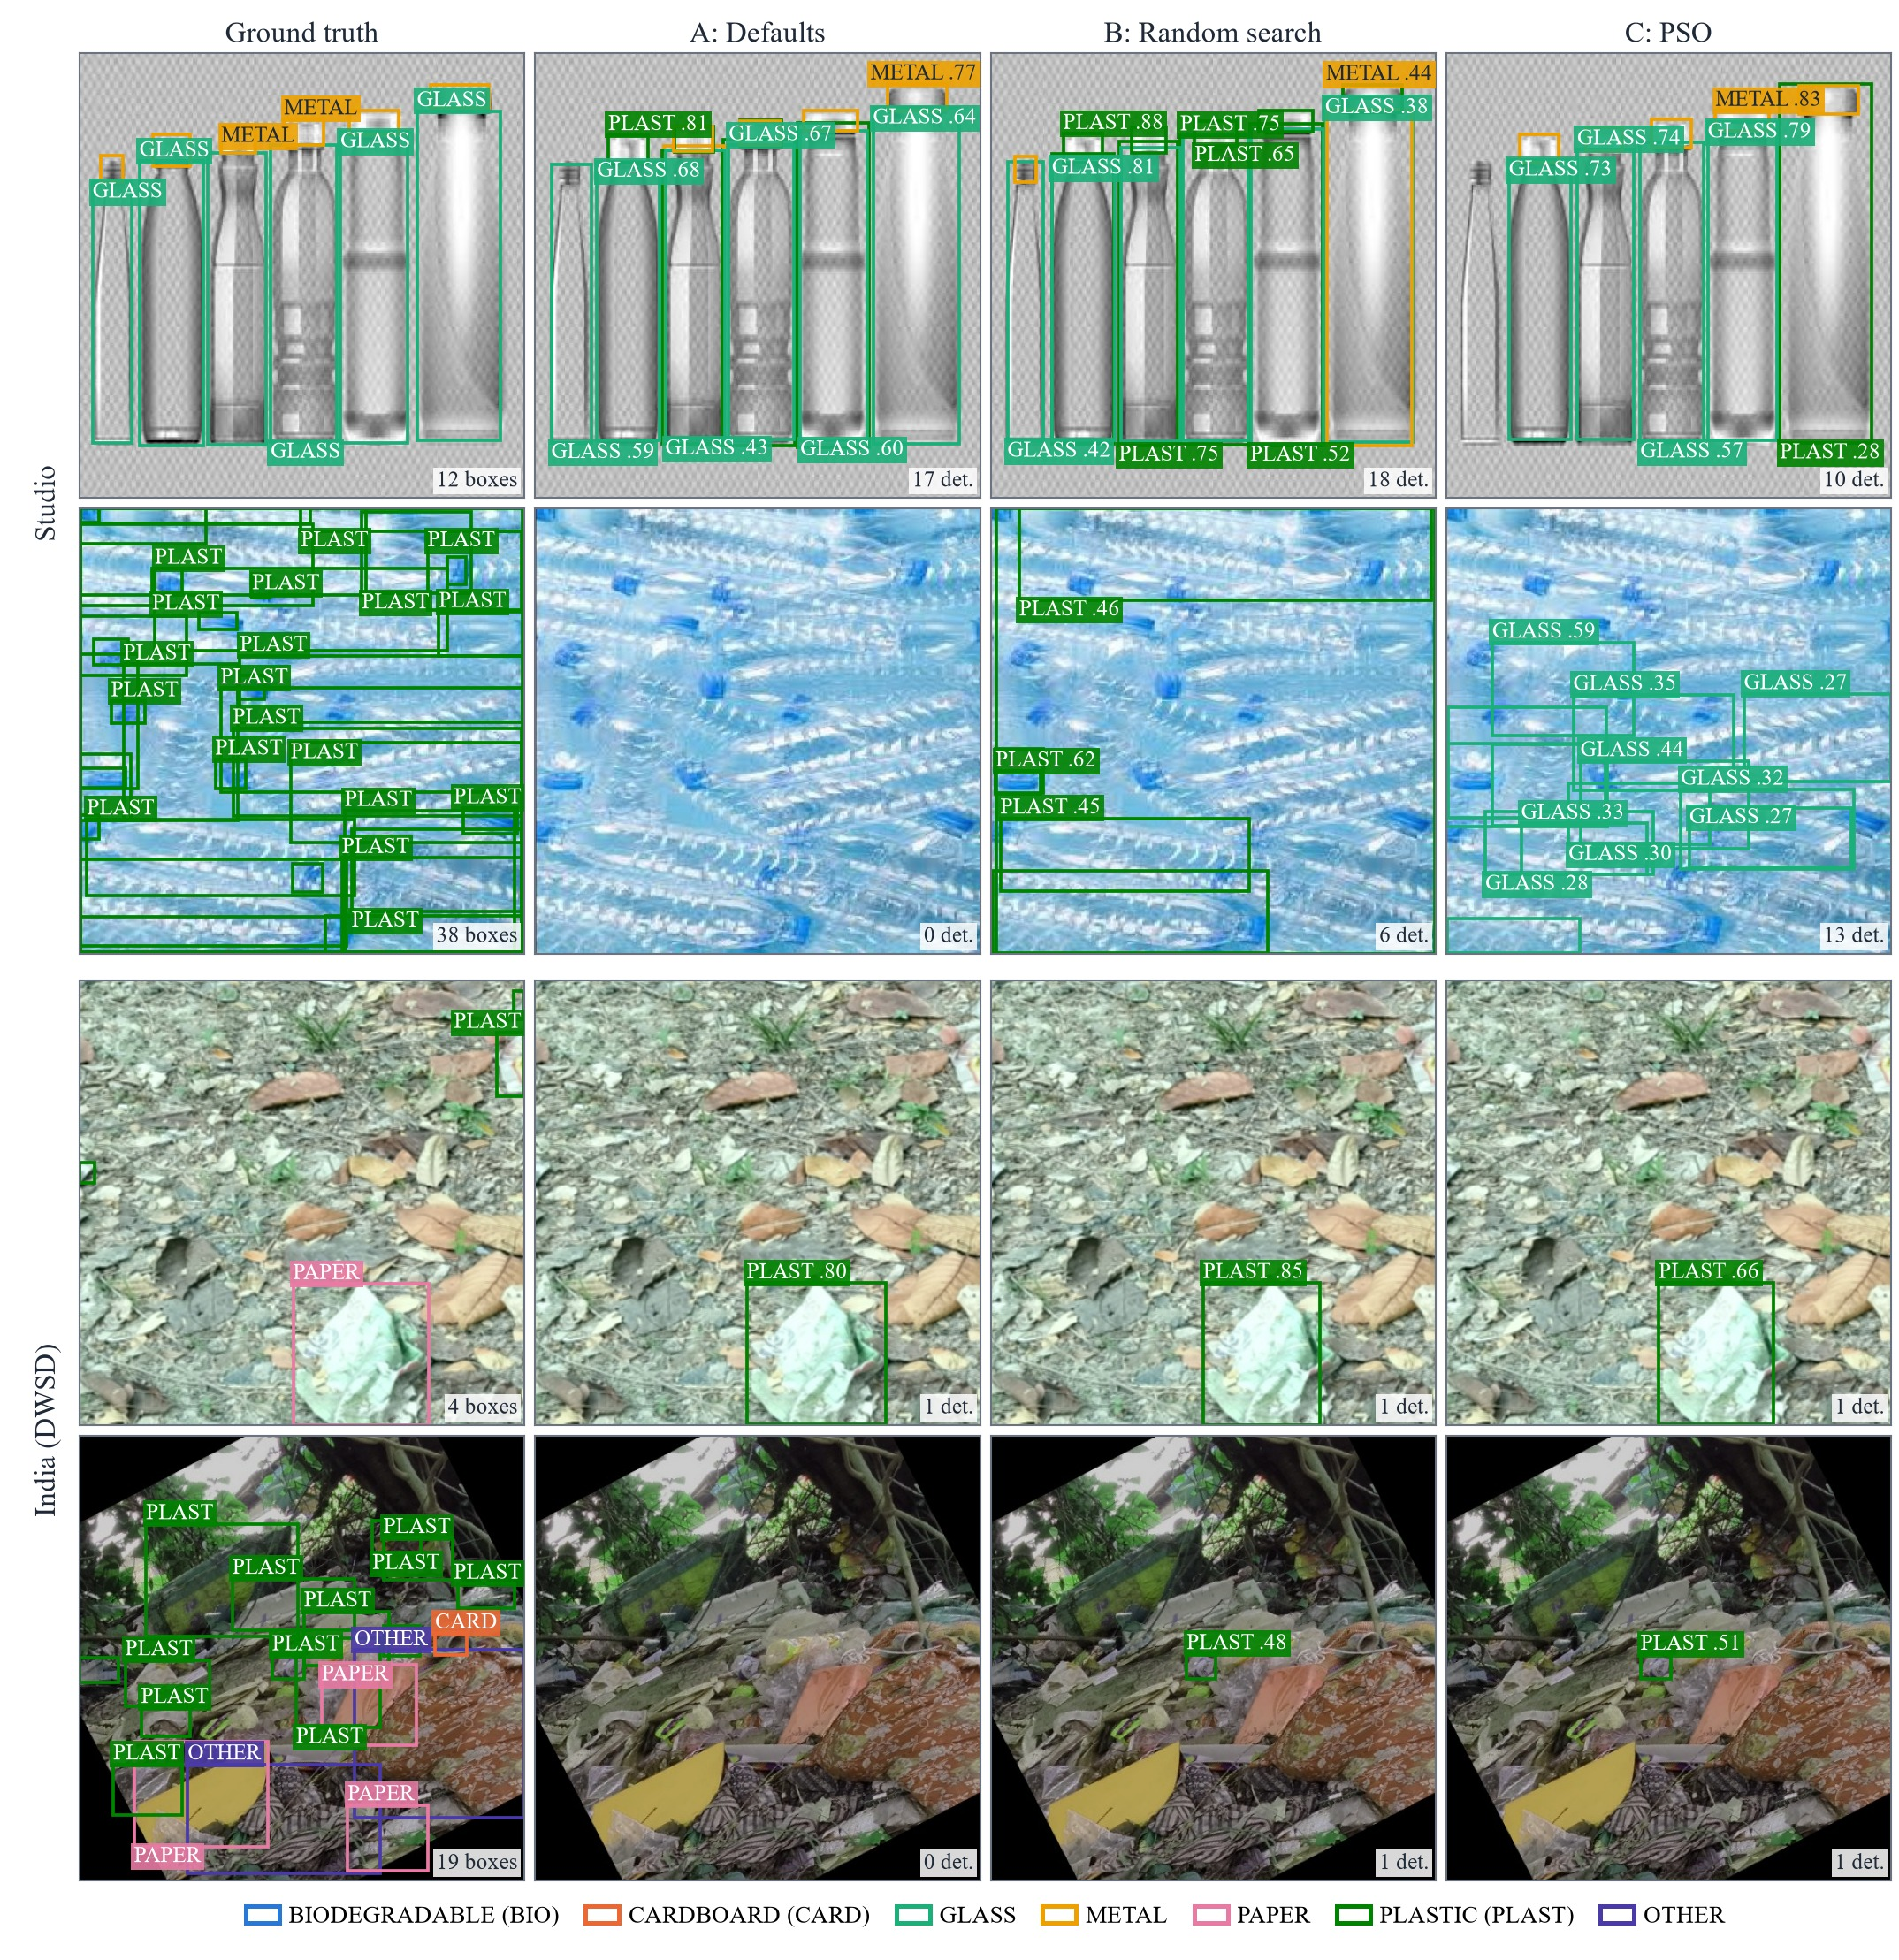
\includegraphics[width=0.85\textwidth]{r_samples.jpg}
\caption{Detections of the three \gentwo models on two studio, two real-world and two Indian (DWSD) test images, next to the ground truth. The images were chosen by a fixed rule, not by eye: for each test set, the images with at least three ground-truth boxes were put in a random order with seed 0, and the first two are shown. Every model saw the same images at 640~px, with a confidence threshold of 0.25 and an NMS IoU of 0.7; the real-world rows show the predictions recorded in the per-image analysis of Fig.~\ref{fig:best}. Each box carries its class and, for predictions, its confidence; a label that would cover another is left out. The corner of each panel gives the number of ground-truth boxes or detections. These panels are illustrations, not evidence; the quantitative results are in Table~\ref{tab:gen2-test} and Fig.~\ref{fig:domains}. The DWSD ground-truth boxes come from mask regions, so touching items of one class can merge into one box.}
\label{fig:samples}
\end{figure*}

The two generations differ in classes, image size and training data, so Tables~\ref{tab:gen1-test} and~\ref{tab:gen2-test} are not one benchmark. Table~\ref{tab:g1g2} therefore scores all six final models on the same studio and real-world test images, restricted to the six shared classes (Section~\ref{subsec:eval}). On the real-world images, every \gentwo arm is significantly better than every \genone arm: 0.338--0.353 \mapfifty against 0.038--0.096, about four to nine times as high. On the studio images, the order reverses: every \genone arm is significantly better than every \gentwo arm, by 0.074 to 0.105. Within each generation, no real-world difference is significant (e.g., \genone C$-$A $+0.048$ [$-0.020$, $+0.163$], \gentwo C$-$B $+0.013$ [$-0.019$, $+0.042$]), and the studio verdicts match Tables~\ref{tab:gen1-test} and~\ref{tab:gen2-test}. The 0.096 of \genone C and its wide interval come largely from the single real-world BIODEGRADABLE box, on which it scores 0.332 AP@50. \gentwo scores higher on real-world images here than in Table~\ref{tab:gen2-test} (A 0.353 against 0.310) only because OTHER is left out of the mean. As a check, \genone reproduces its own studio test result within 0.0004 \mapfifty.

\begin{table}[!t]
\centering
\caption{\genone versus \gentwo on the Same Test Images: Test \mapfifty [95\% CI] on the Six Shared Classes}
\label{tab:g1g2}
\footnotesize
\begin{tabular}{@{}lcc@{}}
\toprule
Model (px) & Real-world (468 img.) & Studio (1,046 img.) \\
\midrule
G1 A (416) & 0.047 [0.038, 0.080] & 0.676 [0.641, 0.719] \\
G1 B (416) & 0.038 [0.031, 0.069] & 0.672 [0.636, 0.716] \\
G1 C (416) & 0.096 [0.041, 0.214] & 0.669 [0.628, 0.716] \\
\midrule
G2 A (640) & 0.353 [0.315, 0.504] & 0.571 [0.529, 0.619] \\
G2 B (640) & 0.338 [0.304, 0.473] & 0.595 [0.557, 0.639] \\
G2 C (640) & 0.352 [0.315, 0.485] & 0.590 [0.550, 0.635] \\
\midrule
$\Delta$ G2$-$G1 & $+0.243$ to $+0.315$ & $-0.105$ to $-0.074$ \\
\bottomrule
\end{tabular}
\\[2pt]
\parbox{\columnwidth}{\footnotesize G1, G2: \genone, \gentwo; each model was scored once at its own training image size (px). Real-world: 647 boxes after removing OTHER, with a single BIODEGRADABLE box; studio: 7,413 boxes, no OTHER. CIs: 1,000 paired bootstrap resamples per test set. $\Delta$: range over all nine G2$-$G1 pairs, every one significant; e.g., real-world G2 B$-$G1 C $+0.243$ [$+0.134$, $+0.418$], studio G2 A$-$G1 A $-0.105$ [$-0.125$, $-0.084$]. On the five real-world classes with more than one box, \gentwo scores 0.239--0.618 AP@50 and \genone 0.008--0.117.}
\end{table}

Where, then, do the \gentwo models succeed on real-world photographs? A per-image analysis of the 468 real-world test images counts an image as fully correct when every ground-truth object is matched by a detection of the same class with IoU $\geq 0.5$ (greedy, highest confidence first, at a confidence threshold of 0.25) and no detection is left unmatched. Each model is fully correct on 166 (A), 168 (B) and 170 (C) images, 35 to 36\% of the set, and all three on the same 111. The successes are almost all single-object photographs: of the 375 images with one object, the models are fully correct on 164 to 167; of the 47 with two objects, on 1 to 4; and of the 46 with three or more, on none. Fig.~\ref{fig:best} shows the most favorable cases, chosen by a fixed rule. No image with three or more objects, and only one with two, is fully correct for all three models, so the rule fell back to the two images with at least two objects that at least two models label fully correctly; one of them is a close-up on a plain background, close to studio conditions. The models thus handle an isolated item in a real scene, but not a cluttered scene with several items.

\begin{figure*}[!t]
\centering
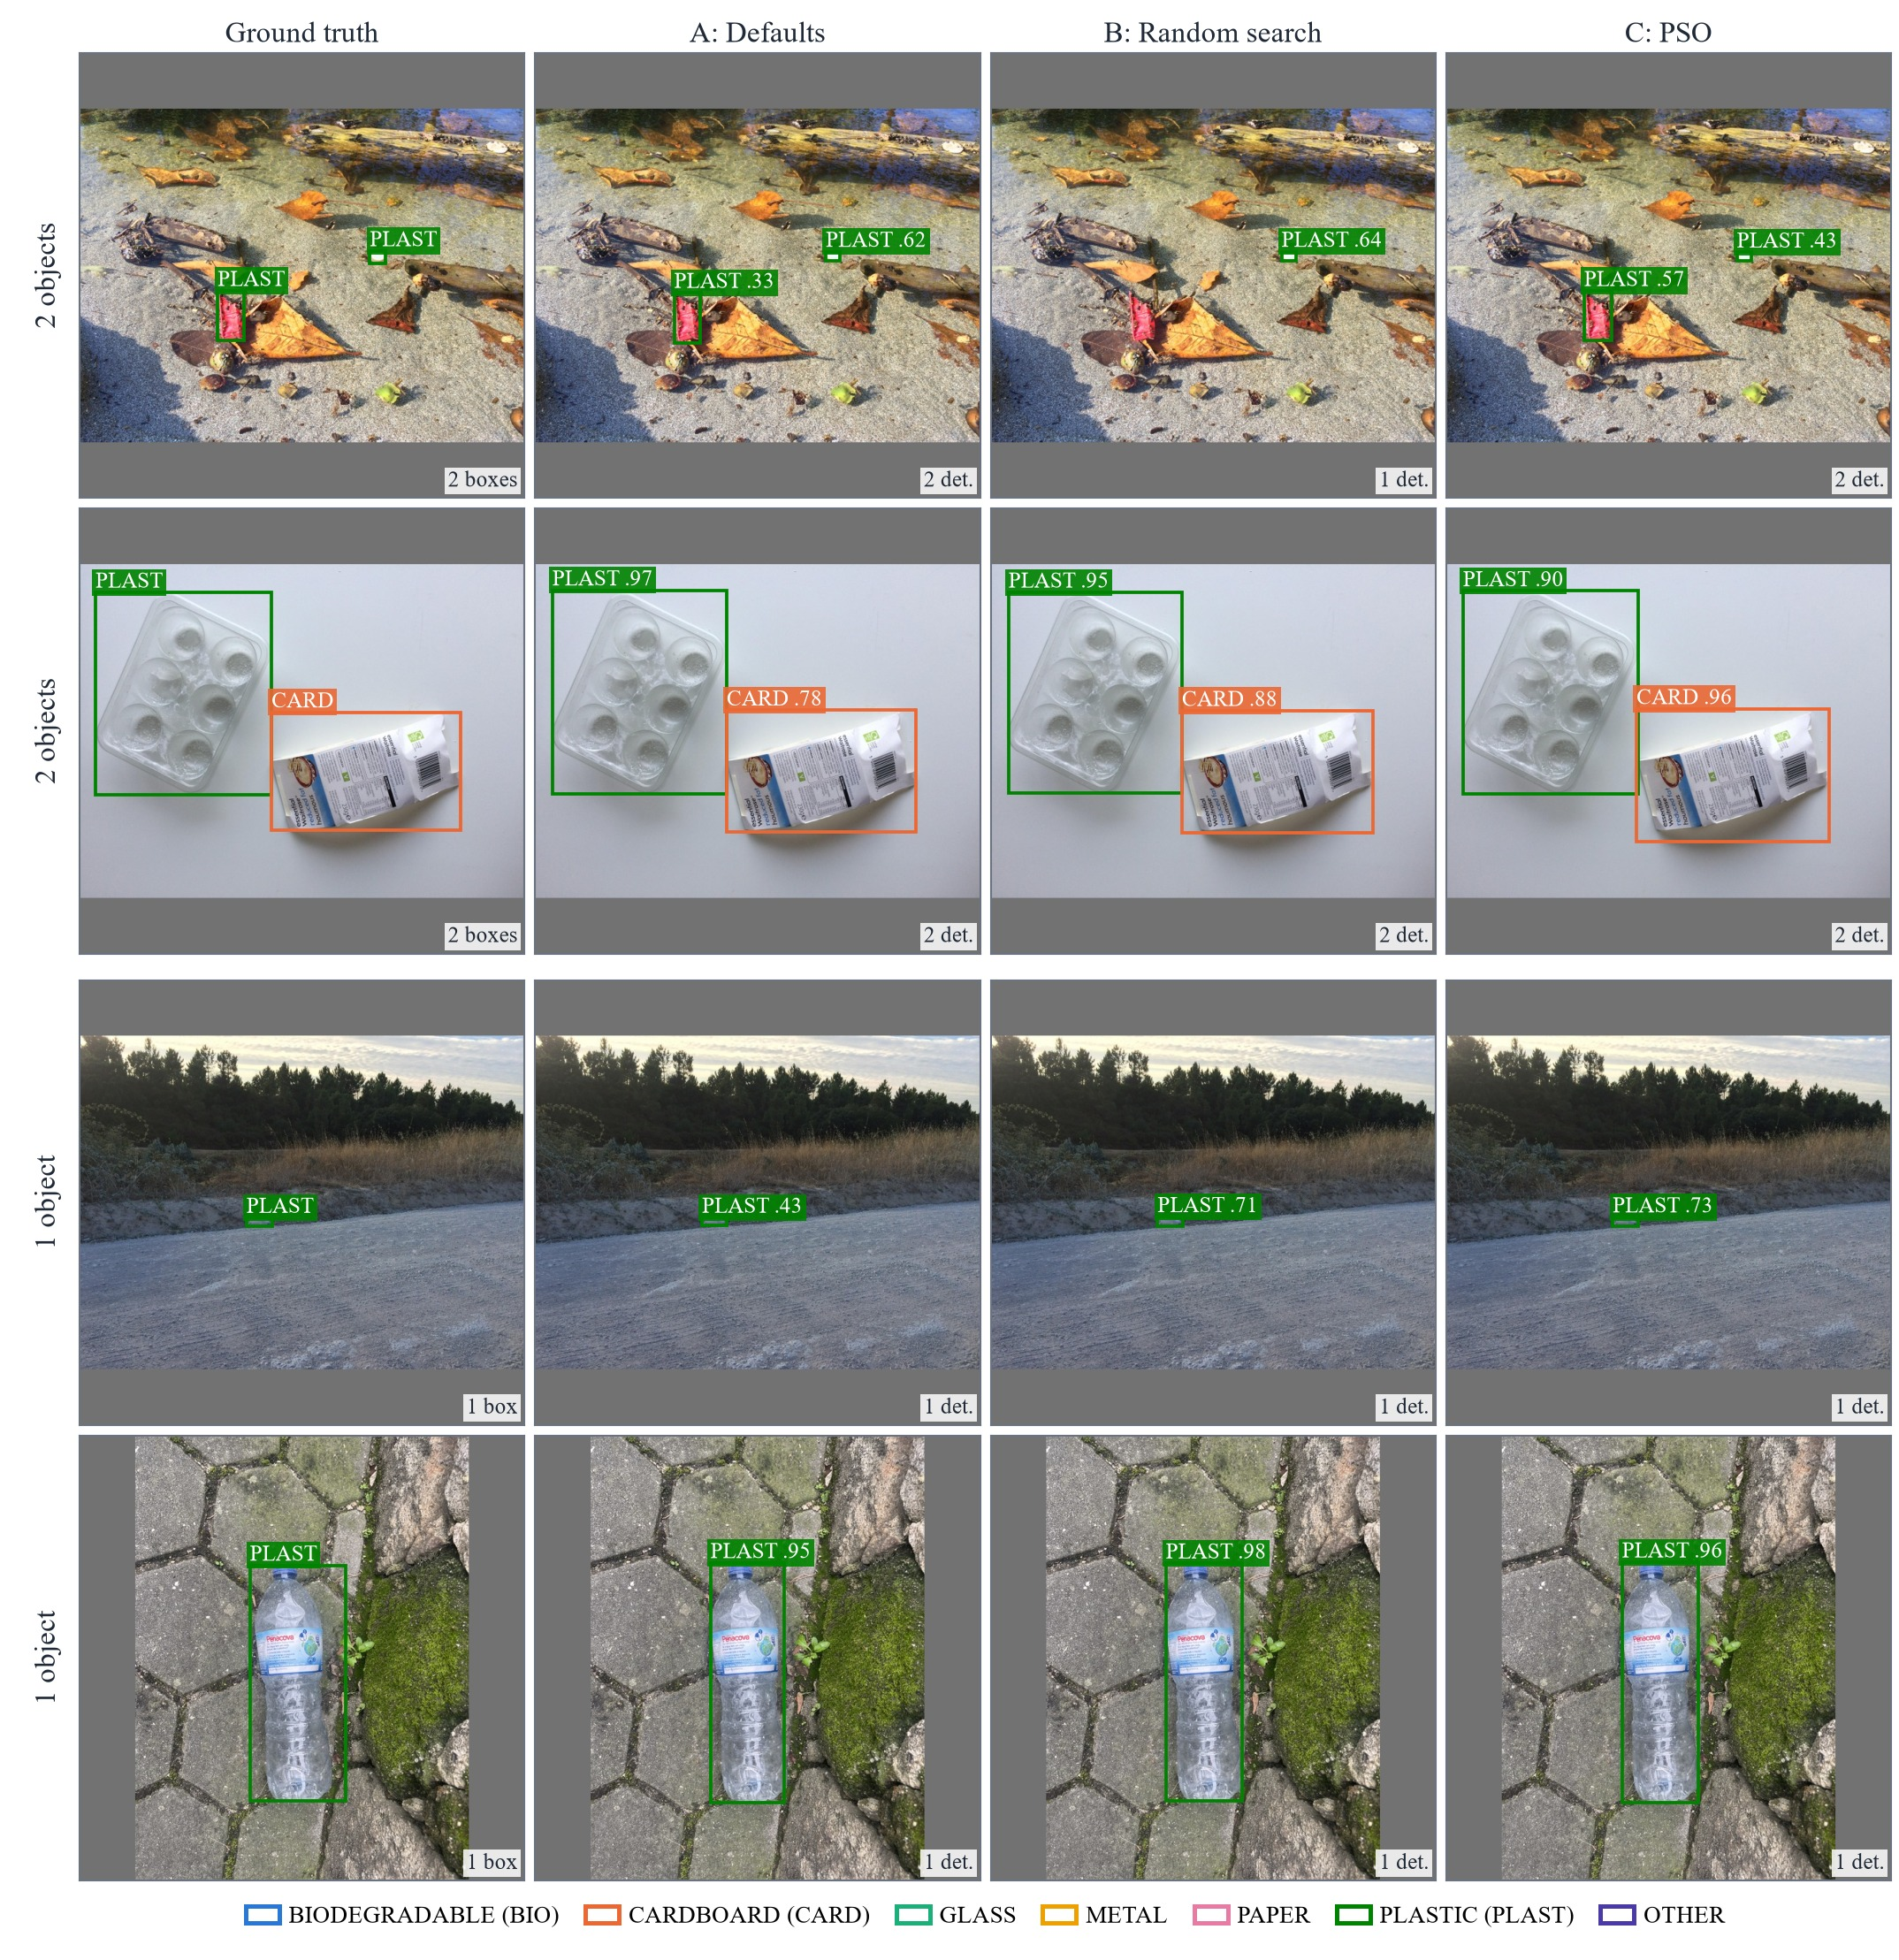
\includegraphics[width=0.8\textwidth]{r_best.jpg}
\caption{Selected success cases on real-world test images: deliberately favorable, not representative. Rows 1--2: the only real-world test images with at least two objects that at least two of the three \gentwo models label fully correctly (every object found with the right class, no false detection); no image with three or more objects qualifies, and random search (B) misses one object in the first. Rows 3--4: the first two of the 110 single-object images that all three models label fully correctly, in a random order with seed 0. Confidence threshold 0.25, NMS IoU 0.7, 640~px. For scale, each model is fully correct on 166--170 of the 468 real-world test images, on 164--167 of the 375 single-object images and on none of the 46 images with three or more objects.}
\label{fig:best}
\end{figure*}

\subsection{Compute Cost}
\label{subsec:res-cost}

Table~\ref{tab:compute} lists the recorded GPU time of every run on one Tesla T4, covering training only (setup, data copies and idle time are excluded). Including its search, each tuned arm cost about 2.7 to 2.8 times the GPU time of Arm~A, which needs no search. The budget was equal in evaluations, not in time: the mean proxy training took 214.3~s for PSO and 238.7~s for random search in \genone, and 285.5~s and 259.0~s in \gentwo. The largest \genone item was the proxy-validity check, of which the eight 40-epoch medium runs took 3.84 of 4.36 hours. In \gentwo, about 24 further GPU-hours were lost when two sessions froze and sat idle until the platform's 12-hour limit; they are not in the totals. The one-time test evaluation took 283.1~s on the laptop CPU in \genone and 220.6~s on the T4 for the four \gentwo test sets.

\begin{table}[!t]
\centering
\caption{Recorded GPU Time per Run (Hours, One Tesla T4)}
\label{tab:compute}
\footnotesize
\begin{tabular}{@{}lcc@{}}
\toprule
Run & \genone & \gentwo \\
\midrule
Proxy-validity check (16 runs) & 4.36 & not run \\
PSO search (32 proxy trainings) & 1.91 & 2.54 \\
Random search (32 proxy trainings) & 2.12 & 2.30 \\
Arm~A full training (100 epochs) & 1.18 & 1.56 \\
Arm~B full training (100 epochs) & 1.15 & 2.07 \\
Arm~C full training (100 epochs) & 1.45 & 1.60 \\
\midrule
Total recorded & 12.18 & 10.06 \\
\bottomrule
\end{tabular}
\\[2pt]
\parbox{\columnwidth}{\footnotesize Sums of the recorded training wall-clock times. The \gentwo random search and Arm~C training were resumed after a session froze (Arm~C after epoch 55); their idle time, about 24 GPU-hours in total, is not included.}
\end{table}
